% ---------------------------------------------------------------------------------
% Figures placed in the free space of page 3 (confusion matrices + error examples),
% generated by Lab4_final_inference.ipynb from the final checkpoints.
% The error examples are cropped one by one from figures/errors_grid.png with
% trim (2880x600 px at 300 dpi, 1 px = 0.24 bp) and their labels are typeset in
% LaTeX, so the text stays legible however small the photos are.
% ---------------------------------------------------------------------------------
\setlength{\intextsep}{4pt}
% \errimg{left trim}{right trim}: one 427x427 px photo of errors_grid.png
\newcommand{\errimg}[2]{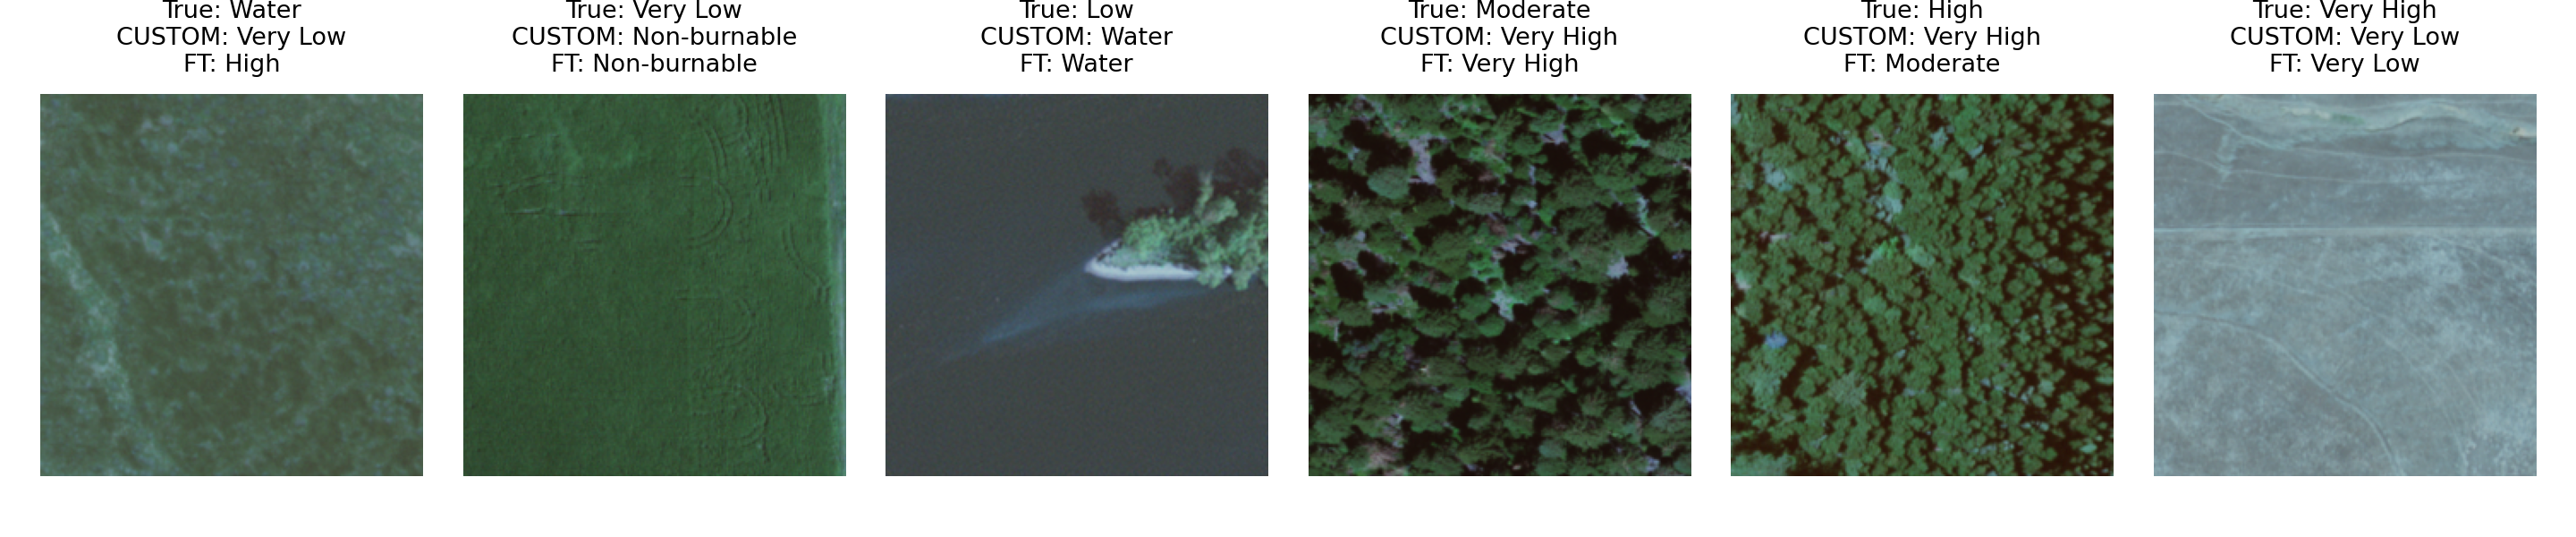
\includegraphics[width=\linewidth,trim=#1 16.32 #2 25.20,clip]{figures/errors_grid.png}}
\begin{figure}[H]
\centering
\begin{minipage}[b]{0.40\linewidth}\centering
\begin{subfigure}[b]{0.49\linewidth}\centering
  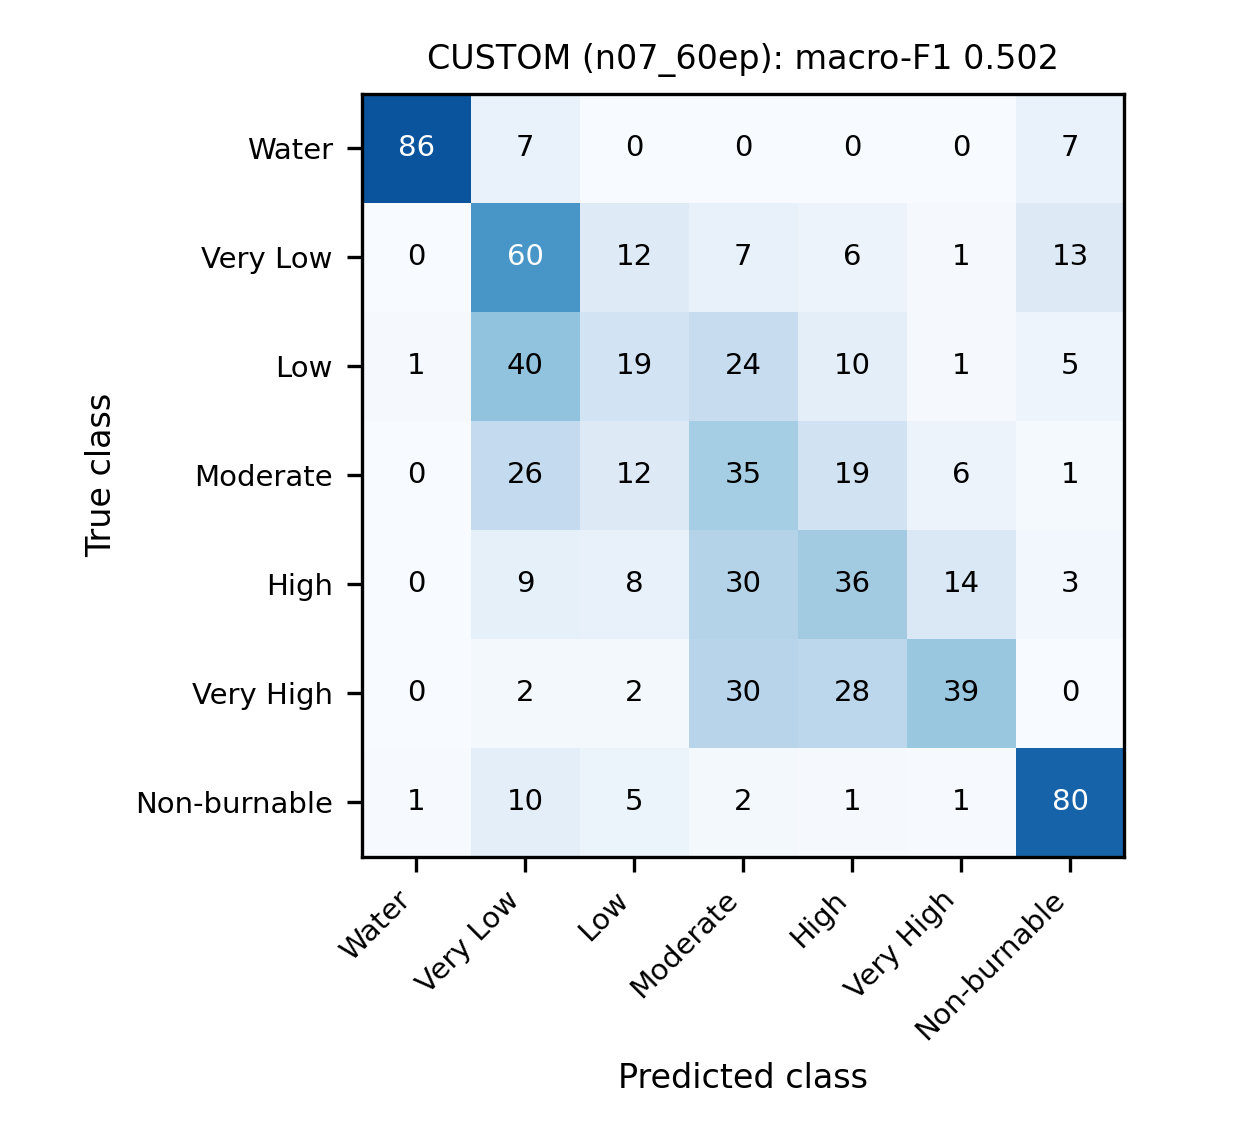
\includegraphics[width=\linewidth]{figures/confusion_custom.png}
  \caption{CUSTOM}
\end{subfigure}\hfill
\begin{subfigure}[b]{0.49\linewidth}\centering
  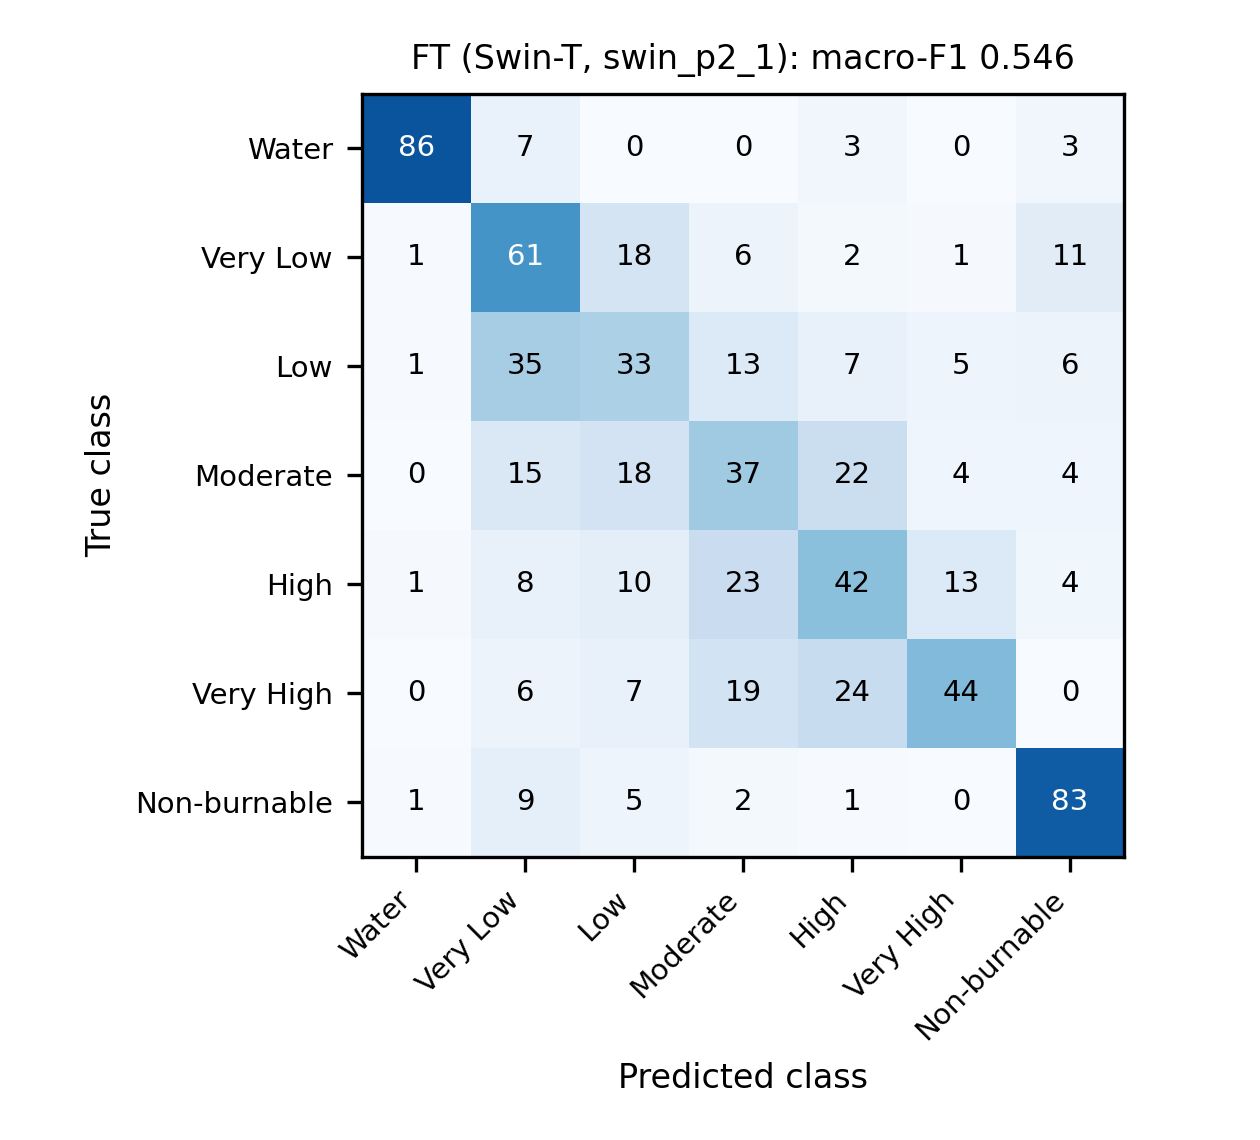
\includegraphics[width=\linewidth]{figures/confusion_ft.png}
  \caption{FT (Swin-T)}
\end{subfigure}
\caption{Validation confusion matrices ($224\times224$ centre crop), row-normalised (\%); rows: true, columns: predicted.}
\label{fig:cm}
\end{minipage}\hfill
\begin{minipage}[b]{0.585\linewidth}\centering
{\fontsize{5.5}{6.2}\selectfont
\setlength{\tabcolsep}{0.8pt}\renewcommand{\arraystretch}{0.9}
\begin{tabular}{@{}r*{6}{>{\centering\arraybackslash}p{0.142\linewidth}}@{}}
 & \errimg{10.80}{577.68} & \errimg{124.32}{464.16} & \errimg{237.60}{350.88}
 & \errimg{351.12}{237.36} & \errimg{464.40}{124.08} & \errimg{577.92}{10.56} \\
\textbf{True} & \textbf{Water} & \textbf{Very Low} & \textbf{Low} & \textbf{Moderate} & \textbf{High} & \textbf{Very High} \\
CUSTOM & Very Low & Non-burnable & Water & Very High & Very High & Very Low \\
FT & High & Non-burnable & Water & Very High & Moderate & Very Low \\
\end{tabular}}
\caption{Errors shared by both models: per true class, the one with the most confident FT prediction (chosen automatically).}
\label{fig:errors}
\end{minipage}
\end{figure}
